\documentclass[10pt,a4paper]{article}
\usepackage[T1]{fontenc}
\usepackage[utf8]{inputenc}
\usepackage[brazil]{babel}
\usepackage{lmodern}
\usepackage[margin=1.45cm,top=1.2cm,bottom=1.3cm]{geometry}
\usepackage{microtype}
\usepackage{booktabs}
\usepackage{graphicx}
\usepackage{array}
\newcolumntype{P}[1]{>{\raggedright\arraybackslash}p{#1}}
\usepackage{titlesec}
\usepackage{enumitem}
\usepackage{siunitx}
\usepackage[hidelinks]{hyperref}
\sisetup{output-decimal-marker={,},group-separator={\,},group-minimum-digits=4}
\titleformat{\section}{\normalsize\bfseries}{\thesection.}{0.4em}{}
\titlespacing*{\section}{0pt}{5pt}{2pt}
\setlength{\parindent}{0pt}
\setlength{\parskip}{2.5pt}
\setlist{nosep,leftmargin=1.1em}
\setlength{\tabcolsep}{4pt}
\pagestyle{empty}
\newcommand{\campo}[1]{\underline{\makebox[#1]{}}}

\begin{document}

{\large\bfseries Tutoria — Processamento Paralelo: OpenMP e CUDA · Relatório}\\[1pt]
{\small Marcelo Gomes Barbosa · Programa de Pós-Graduação em Computação Aplicada (PPCA/UFRR) · Arquitetura e Organização de Computadores · Prof.\ Herbert O.\ Rocha · 24/11/2026}

\vspace{2pt}
\fbox{\parbox{\dimexpr\textwidth-2\fboxsep-2\fboxrule}{\small
\textbf{Predições do discente}\quad P1: \textbf{(a)} sempre correto\quad P2: \textbf{(a)} esgotar os núcleos\quad P3: \textbf{(b)} cerca de metade\\[3pt]P4 (o que acontece em FP64?): \textbf{tudo fica igual}: só mais lento, e os kernels continuam limitados por memória.}}

\section{Ambiente e método}
Sem acesso a uma RTX~3090, a coleta foi feita em duas máquinas. \textbf{Todo número da 3090 citado aqui é o modelo do roteiro, não uma medição.}
As fontes do kit foram usadas sem alteração (sha256 conferido). Todos os scripts, logs brutos e CSVs estão em \href{https://github.com/marcelobns/paralelo-openmp-cuda}{\texttt{github.com/marcelobns/paralelo-openmp-cuda}}.

{\small
\begin{tabular}{@{}P{2.0cm}P{7.9cm}P{7.7cm}@{}}
\toprule
 & \textbf{CPU} — Blocos 1–2 & \textbf{GPU} — Blocos 1, 3 e 4 (Google Colab) \\
\midrule
Máquina & Apple M5: 4 núcleos P + 6 E, 16~GiB de memória unificada (153~GB/s nominais), macOS 27.2.1, na tomada &
Tesla T4 (sm\_75, 40 SM, 320~GB/s, PCIe 3.0 x16), driver 580.82, CUDA 13.0; host Xeon 2,0~GHz com 2 vCPU \\
Compilação & Apple clang 21 + libomp 23.1.5, \texttt{-O3 -mcpu=native}; o Makefile usa gcc &
gcc 13.3 \texttt{-O3 -march=native -fopenmp}; \texttt{nvcc -O3 -arch=sm\_75} em vez de \texttt{sm\_86} \\
Repetições & 15 por ponto, em rodadas intercaladas; \texttt{race} executado 50 vezes; mediana e faixa &
5 por configuração, também com \texttt{CUDA\_MODULE\_LOADING=EAGER}; \texttt{race} executado 50 vezes \\
\bottomrule
\end{tabular}}

{\footnotesize\texttt{verifica\_ambiente.sh} no Colab: gcc com OpenMP OK · 2 núcleos · nvcc 13.0 · Tesla T4, 15360~MiB, 580.82.07.
Kernel: \texttt{node:24.18-alpine} (Node 24.18.1, V8 13.6, Alpine 3.24.1/musl) sob OrbStack no mesmo M5 (VM de 10 vCPU e 4,9~GB), com carga de 0,12 por núcleo.}

\section{Medições (Blocos 1–4)}
\textbf{Bloco 1 — corrida.} Com 4 threads, o mesmo fonte errou em \textbf{100\%} das 50 execuções no M5 e em \textbf{96\%} na VM da T4; o roteiro relata 10\%.
Todo valor errado é uma soma de blocos inteiros: 1\,499\,994–1\,500\,003 é a soma de um bloco de $5\cdot10^5$ iterações, e 3,0 e 4,5 milhões são dois e três blocos.
O assembly do gcc e o do clang são equivalentes: cada thread lê \texttt{soma} uma vez antes do laço e grava uma vez depois, então vence a última gravação.
O resultado só sai certo se as quatro janelas de leitura e gravação não se sobrepuserem. A taxa de erro é uma propriedade do escalonamento, não do código: ``testei e funcionou'' não prova nada.
Com \texttt{reduction(+:soma)}, as 50 execuções no M5 saíram corretas.

\textbf{Bloco 2 — SAXPY OpenMP no M5} ($N=5\cdot10^7$, 0,6~GB por execução; mediana de 15):\\[1pt]
{\small\begin{tabular}{@{}lrrrrrrrr@{}}
\toprule
threads & 1 & 2 & 3 & 4 & 6 & 8 & 10 & 16 \\
GB/s & 62,7 & 91,5 & 106,5 & 110,8 & 119,3 & 121,3 & \textbf{126,8} & 124,7 \\
\bottomrule
\end{tabular}}\quad
\parbox[b]{7.3cm}{\small Ganho máximo de $2{,}0\times$. Com 3 threads o SAXPY já atinge 84\% da banda máxima, e 95\% com \textbf{7 threads}. O teto de 126,8~GB/s é 83\% do nominal.}\\[1pt]
O SAXPY para de escalar pela banda, não pela contagem de núcleos.
Duas ressalvas: a partir de 5 threads entram os núcleos E, e o \texttt{schedule(static)} divide o laço em partes iguais; além disso, com 1 thread a banda variou de 21,8 a 65,7~GB/s, provavelmente por alternância entre núcleos P e E.
O teste com $N=2\cdot10^8$ teve coeficiente de variação de 30–40\%, ruidoso demais para entrar na tabela; os picos individuais (130~GB/s) confirmam o teto.

\textbf{Bloco 3 — PCIe na T4} ($N=10^8$; mediana de 5; faixa da fração entre parênteses):\\[1pt]
{\small\begin{tabular}{@{}lrrrrr@{}}
\toprule
 & H$\to$D & kernel & D$\to$H & total & \% em transferência \\
\midrule
1 repetição & 175,1 ms (4,6 GB/s) & 5,45 ms (220 GB/s) & 91,9 ms (4,4 GB/s) & 272,4 ms & \textbf{98,0} (98,0–98,3) \\
50 repetições & 173,3 ms & 266,5 ms (225 GB/s) & 92,3 ms & 531,2 ms & \textbf{50,2} (49,8–50,6) \\
\bottomrule
\end{tabular}}\\[1pt]
A transferência custou $49\times$ o kernel. O roteiro prevê $39\times$ para a 3090, e o modelo da T4 a 12~GB/s prevê $27\times$.
O PCIe entregou só 38\% do suposto, provavelmente porque a memória do host é paginável (\texttt{malloc}) e a máquina é virtual.
Recalculado com as taxas medidas, o modelo prevê 98,0\% e 49,5\%; os valores medidos foram 98,0\% e 50,2\%.
Pagar a transferência contra o pico FP32 exigiria \num{21237} FLOP por elemento; o SAXPY faz 2.
O teste com \texttt{EAGER} deu $\text{kernel}_{1\times}/(\text{kernel}_{50\times}/50)=1{,}02$, ou seja, não há custo de primeira chamada.

\textbf{Bloco 4 — roofline da T4.} Picos de 8,14~TFLOP/s em FP32 e 0,25 em FP64 (1/32), com 320~GB/s; o equilíbrio é de 25,4 e 0,80~FLOP/B.
O SAXPY medido faz 37,5~GFLOP/s, \textbf{0,46\% do pico FP32} (0,44\% no modelo da 3090) e 70\% do teto de banda.
A inversão do roteiro se repete: o matmul com tile é limitado por memória em FP32 (31\% do pico) e atinge 100\% do pico em FP64, onde o limite passa a ser o cômputo.

\section{Kernel da dissertação: cadeia do wake word em \texttt{node:24.18-alpine}}
\textbf{O que foi testado.} A dissertação (pré-projeto, PPCA) usa o Diagrama como instrumento: ditado $\to$ STT $\to$ LLM $\to$ campos. A extração por LLM roda na \texttt{api} e no provedor remoto, sem FLOP local a medir.
O kernel testado é a \textbf{cadeia de wake word} do openWakeWord (\texttt{web/lib/wakeword.ts}), o caminho quente da voz, executada a cada passo de 80~ms: melspectrograma $\to$ embedding (CNN) $\to$ classificador, em onnxruntime-web 1.27 (wasm, FP32).
Ela foi medida na imagem \texttt{node:24.18-alpine} dos estágios \texttt{deps} e \texttt{runner}, com o mesmo runtime do navegador (wasm puro, que funciona sob musl), e validada nos 48 clipes do \texttt{vozes.v1}.
Em produção a cadeia roda no navegador (ADR-003; em \texttt{wakeword.ts}, ``o áudio ocioso nunca sai do dispositivo''); rodá-la no \texttt{runner} exigiria enviar esse áudio ao servidor.

\textbf{Contagem.} FLOP por nó, lidos dos grafos ONNX com as formas reais: Conv $=2\,C_\text{out}\,|\text{saída}|\,C_\text{in}k$, MatMul/Gemm $=2MNK$ e 1 FLOP por elemento nas operações ponto a ponto.
O mel é uma STFT feita por duas Conv1D (janela 512, passo 160) sobre 1,2~s de áudio (117 quadros), seguida de um MatMul para 32 bandas.
Bytes: o compulsório é pesos + entrada + saída (4~B cada), que dá a AI máxima; sem reuso, cada operador lê e grava seus tensores, o que dá a AI mínima.

\noindent\begin{minipage}[c]{0.555\textwidth}
{\footnotesize\setlength{\tabcolsep}{3pt}\begin{tabular}{@{}lrrrr@{}}
\toprule
por passo de 80 ms, 1 thread & MFLOP & AI (FLOP/B) & tempo & GFLOP/s \\
\midrule
mel, janela de 1,2 s & 63,6 & 16,9–54,0 & 1,35 ms & 47,1 \\
embedding $[1,76,32,1]$ & 85,0 & 8,2–64,3 & 2,02 ms & 42,2 \\
classificador $[1,16,96]$ & 0,21 & 0,47–0,49 & 0,018 ms & 11,5 \\
\textbf{cadeia} (pesos 2,8 MB) & \textbf{148,8} & \textbf{10,2–51,0} & \textbf{3,38 ms} & \textbf{44,0} \\
\midrule
mel incremental (8 quadros) & 4,35 & 3,4–4,0 & 0,184 ms & 23,7 \\
cadeia com mel incremental & 89,6 & 7,4–31,6 & 2,22 ms & 40,4 \\
\bottomrule
\end{tabular}}\\[3pt]
{\footnotesize\textbf{Figura ao lado:} roofline empírico do runtime (wasm, 1 thread), com tetos medidos na mesma imagem: MatMul $1024^3$ e cópia nativa de 128~MB (mediana de 9 execuções). Barras: faixa de AI de cada etapa na altura do GFLOP/s medido (mediana de 300 amostras em 5 rodadas intercaladas).}
\end{minipage}\hfill
\begin{minipage}[c]{0.425\textwidth}
\centering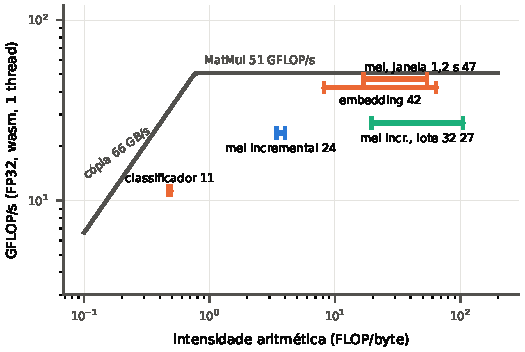
\includegraphics[width=\linewidth]{fig_roofline_wasm.pdf}
\end{minipage}

\section{Diagnóstico de regime e alteração proposta}
Os tetos medidos na imagem são 50,7~GFLOP/s (MatMul) e 66~GB/s (cópia nativa; faixa 41–83, perto dos 62,7 do Bloco 2 com 1 thread), com equilíbrio de 0,76~FLOP/B. O Add do ORT dá só 16~GB/s porque inclui copiar os tensores para o \textit{heap} do wasm, e por isso não serve de teto.
A cadeia tem AI entre 10 e 51 e roda a 44~GFLOP/s, \textbf{87\% do teto: é limitada por cômputo}. O mel chega a 93\% e o embedding a 83\%.
A prova: em lote de 32 fluxos, a AI do embedding sobe até 1663, mas o tempo por fluxo não cai (2,17 contra 2,02~ms), porque os 2,8~MB de pesos já ficam no cache entre passos.
O classificador (AI 0,48) fica abaixo do equilíbrio, a 36\% do teto de banda; seu limite é o custo fixo da chamada (18~µs), e ele pesa só 0,5\% da cadeia.
Com 4 threads, a cadeia cai para 1,51~ms ($2{,}25\times$), e o MatMul escala $2{,}65\times$.
No navegador não há esse ganho, porque, sem os cabeçalhos COOP/COEP (\texttt{next.config.mjs}), não há \texttt{SharedArrayBuffer} e o ORT roda em 1 thread.
\textbf{Proposta: mel incremental.} A cada passo, \texttt{wakeword.ts} recalcula os 117 quadros da janela inteira, mas só 8 são novos: 93\% do trabalho do mel é repetido.
Calcular só os 8 quadros novos sobre 1632 amostras alinhadas à mesma grade, guardando os 76 últimos, \textbf{muda a AI} do mel de 17–54 para 3,4–4,0, porque os 1,09~MB da base da STFT passam a servir 8 quadros, não 117.
Ainda acima do equilíbrio, ele roda a 47\% do teto: com só 8 quadros de saída, cada Conv tem pouco trabalho por chamada (em lote de 32, 53\%).
Medido: o mel cai de 1,35 para 0,18~ms ($7{,}3\times$) e a cadeia de 3,38 para 2,22~ms ($1{,}5\times$; 2,8\% do passo de 80~ms).
A saída muda pouco: o score se afasta em até $2{,}9\cdot10^{-3}$, sem mudar nenhuma decisão (abaixo), provavelmente porque o grafo corta o mel 80~dB abaixo do máximo, que passa a ser o dos 8 quadros. Silêncio digital não foi testado: os clipes têm ruído de fundo a $-60$~dBFS.
Depois disso o embedding é 91\% da cadeia e já roda a 83\% do teto; só restam mais núcleos ou menos FLOP.

\section{Análise de precisão: o FP32 serve?}
O ORT não tem Conv em FP64, então escrevi uma referência FP64 em numpy dos três grafos. Em FP32, ela reproduz o ORT com erro de $10^{-6}$ no mel e $10^{-7}$ no score.
Rodei o laço de \texttt{wakeword.ts} sobre os 48 clipes do \texttt{vozes.v1} (8 com ``Laudomiro'', 40 sem; 3664 passos) na imagem e comparei os resultados com essa referência.
\textbf{FP32 (produção):} $\max|\Delta\text{score}|=2{,}3\cdot10^{-6}$ (mediana $2\cdot10^{-8}$), \textbf{nenhum passo muda de lado no limiar 0,5} e as detecções são idênticas (8/8 e 0/40). A margem é larga: o menor pico positivo é 0,995 e o maior negativo, 0,002.
\textbf{Conclusão: FP32 é aceitável}, e FP64 não acrescentaria nada.
\textbf{Ganho:} o FP32 é o formato que o runtime acelera. O SIMD do wasm (128~bits) faz 4 operações FP32 ou 2 FP64 por instrução, e os bytes dobram em FP64; o SAXPY em JS puro ficou $2{,}3\times$ mais lento em \texttt{Float64Array} (51,8 contra 22,4~ms).
Descer abaixo de FP32 não compensa: o int8 dinâmico deixou o embedding $2{,}8\times$ \emph{mais lento} (5,7~ms) e o score se afastou até 0,19. Com tudo em int8, perde 1 dos 8 positivos.
Na GPU vale o mesmo: o contêiner não tem GPU (Alpine/musl, sem runtime NVIDIA), e no navegador o caminho seria o WebGPU, cuja linguagem (WGSL) não tem FP64. A inversão FP64 do roteiro não se aplica, e o kernel é FP32 de ponta a ponta.

\section{Síntese (Bloco 5)}
{\small\begin{tabular}{@{}P{6.0cm}P{11.6cm}@{}}
\toprule
Ponto de saturação medido no OpenMP & \textbf{7 threads} (95\% da maior mediana; 84\% já com 3) — M5 \\
Banda máxima observada na CPU & \textbf{126,8 GB/s} (mediana de 15; pico individual 130,8; 83\% dos 153 nominais) \\
Fração em transferência, $N=10^8$, 1 repetição & \textbf{98,0\%} (T4, PCIe a 4,6 GB/s) \\
Fração com 50 repetições & \textbf{50,2\%} \\
AI do kernel da dissertação & Cadeia do wake word, FP32: \textbf{10–51 FLOP/B} (mel 17–54; embedding 8–64; classificador 0,5); com mel incremental, 7–32 \\
Limitado por memória ou por cômputo? & \textbf{Por cômputo}: 87\% do teto de 51~GFLOP/s (wasm, 1 thread), com AI acima do equilíbrio de 0,76; o lote de 32 fluxos sobe a AI sem ganho de tempo, e 4 threads dão $2{,}25\times$. No navegador, 1 thread \\
\bottomrule
\end{tabular}}

\end{document}
